\documentclass[twoside,openany]{book} % Use 'book' for double-sided printing
\usepackage[portuguese]{babel}

% Define trim size and bleed
\newlength{\trimwidth}
\newlength{\trimheight}
\setlength{\trimwidth}{6.69in}
\setlength{\trimheight}{9.61in}
\newlength{\bleed}
\setlength{\bleed}{0.125in}
\newlength{\textmargin}
\setlength{\textmargin}{0.5in}
\newlength{\topbottommargin}
\setlength{\topbottommargin}{1in}
\newlength{\innermargin}
\setlength{\innermargin}{0.75in}

% Calculate total paper dimensions
\newlength{\mypaperwidth}
\newlength{\mypaperheight}
\setlength{\mypaperwidth}{\trimwidth} % Base width
\addtolength{\mypaperwidth}{\bleed}   % Add outer bleed
\setlength{\mypaperheight}{\trimheight}
\addtolength{\mypaperheight}{2\bleed} % Add top and bottom bleeds
\usepackage[paperwidth=\mypaperwidth,paperheight=\mypaperheight]{geometry} % Temporary base paper size for compilation

% Set up geometry with asymmetric margins for odd/even pages
\geometry{
  left=\textmargin,
  right=\textmargin,
  inner=\innermargin,
  top=\topbottommargin,
  bottom=\topbottommargin,
}


\usepackage{amsmath}
\usepackage{amsfonts}
\usepackage{tikz}
\usetikzlibrary{arrows.meta, decorations.pathmorphing}

\usepackage{pdfpages}
\usepackage{fancyhdr} % For custom headers/footers (often used in books)
\usepackage{graphicx}
\usepackage{eso-pic}

% --- Custom Header/Footer Setup (Example using fancyhdr) ---
% You might already have this set up in your book's class or style file
\pagestyle{fancy}
\fancyhf{} % Clear all header and footer fields
\fancyhead[LE,RO]{\thepage} % Page number on left even, right odd
%\fancyhead[LO]{\rightmark} % Chapter title on left odd
%\fancyhead[RE]{\leftmark}  % Section title on right even (if using sections)
%\fancyfoot[C]{\textit{Your Author Name}} % Author in the center footer

\renewcommand{\headrulewidth}{0pt} % NO line under header
\renewcommand{\footrulewidth}{0pt} % NO line above footer
% -----------------------------------------------------------


\usepackage{fontspec}
%\setmainfont{Comic Sans MS}
%\setmainfont{Comic Neue}
\setmainfont{Patrick Hand}
%\setmainfont[Ligatures=TeX]{Segoe Print}

\usepackage{hyperref}
\hypersetup{
    colorlinks,
    citecolor=black,
    filecolor=black,
    linkcolor=black,
    urlcolor=black
}

% Define custom page number style
\fancypagestyle{fancy}{
  \fancyhf{} % clear all headers/footers
  \fancyfoot[C]{%
    \tikz[baseline=(n.base)]{
      \node[circle, fill=black, text=white, inner sep=5pt] (n) {\thepage};
    }%
  }
  \renewcommand{\headrulewidth}{0pt} % remove header line
  \renewcommand{\footrulewidth}{0pt} % remove footer line
}

\title{O Grande Hotel Infinita}
\author{Leonardo Araújo}
\date{} 

\begin{document}
\pagenumbering{gobble}
\thispagestyle{empty}
\includepdf[pages=-]{cover.pt.pdf}

\clearpage
\thispagestyle{empty} % No page number on this page
\mbox{} 
\clearpage

%\frontmatter
\pagenumbering{arabic} % start numbering from here
\setcounter{page}{1}
\maketitle
\thispagestyle{empty}

\thispagestyle{empty} % Sem número de página nesta página

\vspace*{\fill} % Empurra o conteúdo para o fundo

\begin{center}
    \textbf{\huge O Grande Hotel Infinita} % Título principal
    
    %\vspace{0.5cm} % Espaço entre o título principal e as informações de copyright
    \large Informações de Direitos Autorais \textcopyright{} 2025 % Adicionado símbolo de copyright e ano
\end{center}

\vspace{1cm}

\begin{flushleft}
    \emph{Autor:} Leonardo Araújo
\end{flushleft}

\vspace{0.5cm}

\begin{flushleft}
    \emph{Licença:} CC BY-NC-SA

    %
\includegraphics[width=2cm]{cc-by-nc-sa.pdf}

    Este trabalho está licenciado sob a \href{https://creativecommons.org/licenses/by-nc-sa/4.0/}{Licença Internacional Creative Commons Atribuição-NãoComercial-CompartilhaIgual 4.0}.

    Para ver uma cópia desta licença, visite \url{https://creativecommons.org/licenses/by-nc-sa/4.0/}.
\end{flushleft}

\vspace{0.5cm}

\begin{flushleft}
    \emph{Atribuições de Imagens:}

    \begin{itemize}
        \item Algumas imagens foram criadas pelo autor, Leonardo Araújo.
        \item Algumas imagens foram obtidas de domínio público ou fontes com licenças semelhantes.
        \item Algumas imagens foram geradas usando ferramentas de Inteligência Artificial (IA).
    \end{itemize}
\end{flushleft}

\vspace*{\fill} % Empurra o conteúdo para o topo
\begin{center}

\includegraphics[width=2cm]{cc-by-nc-sa.pdf}
\end{center}

\newpage


\Large
\tableofcontents % Table of contents

\clearpage
\thispagestyle{fancy}

\includepdf[pages={1},
            pagecommand={\thispagestyle{fancy}}, % Apply your custom 'fancy' style
            fitpaper=true,
            noautoscale
           ]{infinity.pdf}
\clearpage 
\chapter*{Prefácio} % -- Embrace the journey of knowledge}
Você já se perguntou o quão grande é o infinito, ou se um infinito poderia ser maior que outro? Um problema impossível e paradoxal pode ter uma solução perfeitamente lógica? A matemática, com seus números, regras e equações, pode parecer abstrata, mas na verdade é uma ferramenta incrível que nos permite explorar mundos que só existem em nossa imaginação.

Nesta história, você vai mergulhar no mundo do Grande Hotel Infinita. Um lugar onde os números guiam o caminho e o infinito se torna uma perdição. Junte-se a uma garota inteligente e seu fiel amigo de quatro patas para desvendar um mistério que parece impossível. Prepara-se para embarcar em uma aventura fantástica onde o impossível e a matemática se unem, com pitadas de humor, para resolver um problema espinhoso!


%\mainmatter

%\cleardoublepage 
\clearpage
\includepdf[pages={1},
            pagecommand={\thispagestyle{fancy}}, % Apply your custom 'fancy' style
            fitpaper=true,
            noautoscale
           ]{lobby.pdf}
\clearpage
\chapter{O Paradoxo e o Desaparecimento}
\vspace{-2em}
Abrigado no coração de uma cidade glamourosa, um lugar onde os viajantes mais exigentes do mundo vêm para descansar e recarregar as energias, ergue-se um hotel que é ao mesmo tempo um destino e uma cápsula do tempo: o Grande Hotel Infinita. Era um edifício antigo e magnífico, infinitamente alto e largo, onde a história e o luxo se encontravam. Um lugar onde cada hóspede podia escapar das exigências do mundo moderno e reabastecer suas energias em um ambiente de elegância atemporal. Por causa de seu tamanho e idade, o hotel não tinha elevadores de passageiros, apenas uma quantidade infinita de escadas conectando todos os andares. Para proporcionar maior conveniência, o hotel havia instalado recentemente um pequeno e barulhento elevador de carga conectado a cada quarto. Os hóspedes podiam ligar para a recepção para pedir lanches, bebidas ou toalhas limpas, e seu pedido seria entregue através do elevador de carga.

O saguão, com tetos altíssimos, apresentava uma grande escadaria de mármore que parecia subir para sempre. Um enorme lustre lançava uma luz quente e dourada, criando uma atmosfera encantadora. A recepção era uma obra-prima de mogno esculpido, gerida por funcionários em uniformes impecáveis. Na recepção, sentava-se Henrietta, uma hipopótamo de bom coração. Seu assistente, Bernard, um rato mensageiro diligente, esperava ao lado com carrinhos de bagagem polidos, aguardando o próximo hóspede. Eles eram os dois únicos funcionários do hotel. Com um número infinito de quartos para manterem em ordem, eles tinham que lidar com um fluxo interminável de hóspedes chegando e partindo a toda hora. Era um dever que cumpriam com maestria, graças à sua organização impecável e ao compromisso com a harmonia.

\clearpage
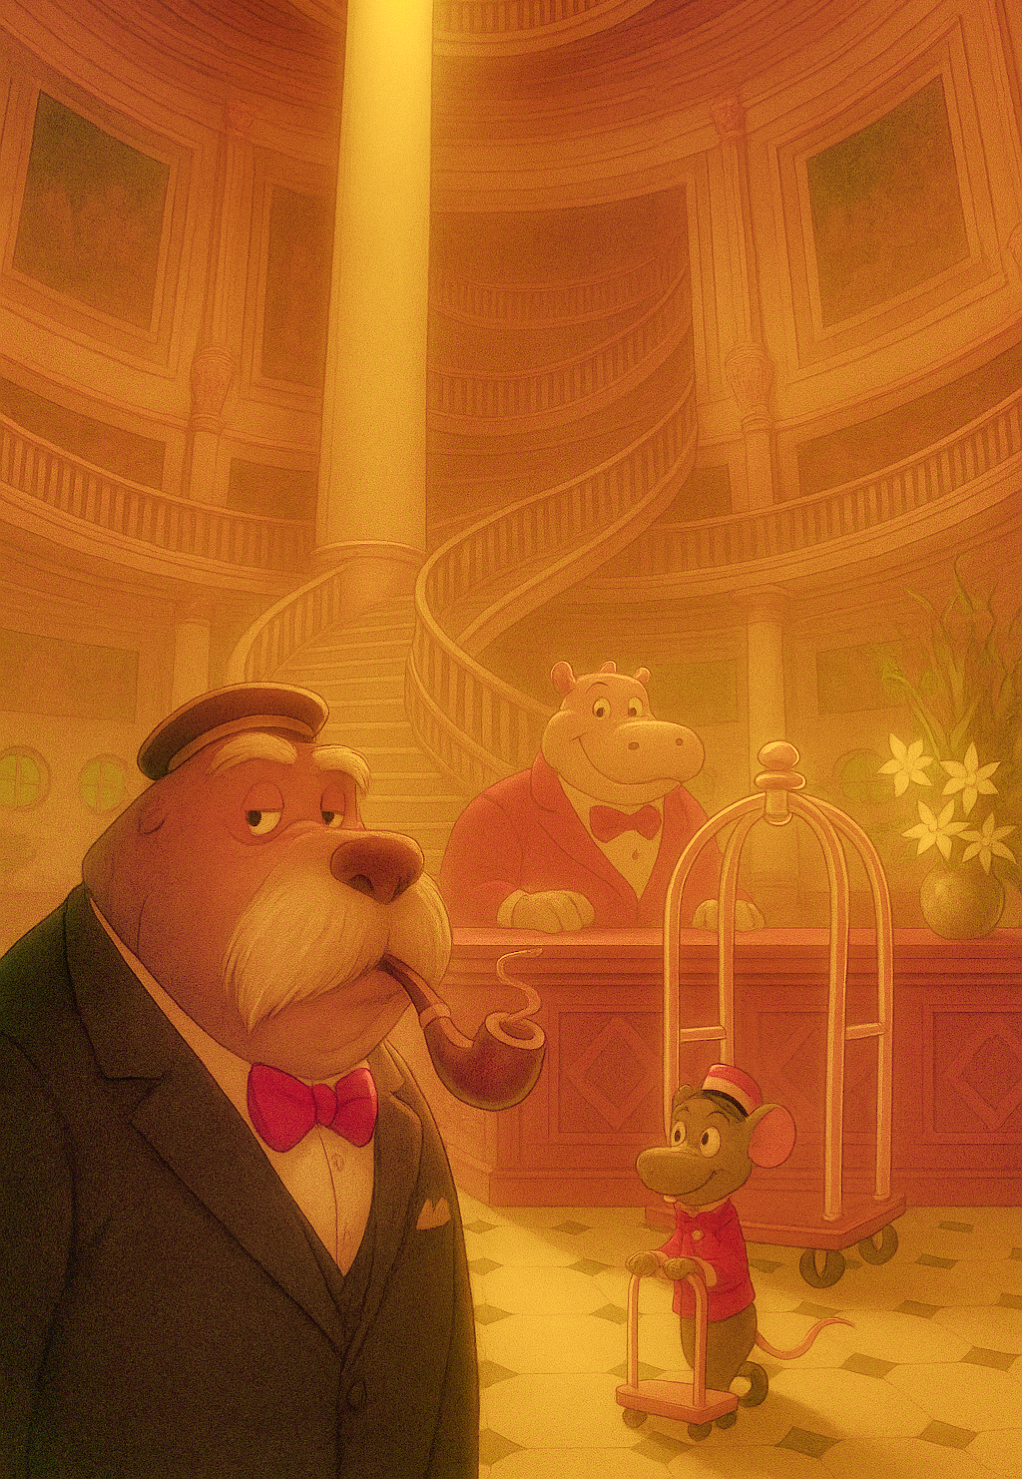
\includepdf[pages={1},
            pagecommand={\thispagestyle{fancy}}, % Apply your custom 'fancy' style
            fitpaper=true,
            noautoscale
           ]{walrus.pdf}

Na noite anterior ao feriado, um distinto leão-marinho fumando um cachimbo foi o último hóspede a chegar. Ele parecia terrivelmente cansado ao entrar. Henrietta, sempre acolhendo os novos hóspedes com afeto, o cumprimentou com um sorriso largo.

``É um prazer recebê-lo no Grande Hotel Infinita'', ela disse. ``Um lugar onde a busca incessante se desfaz, para que você descanse e encontre paz.''
%``Um lugar onde a busca incessante fica para trás, onde você pode descansar e deixar o redemoinho dos turbulentos sonhos para trás.''

``Oh, é tudo que eu preciso'', o leão-marinho respondeu com um suspiro de alívio.

``Nosso hotel está bem cheio hoje, mas o senhor está com sorte, Sr. Leão-Marinho! O primeiro quarto no primeiro andar acaba de ficar vago!'' Henrietta exclamou. ``Nosso ágil Bernard irá ajudá-lo a chegar ao seu quarto imediatamente.''

Bernard o levou ao seu quarto, onde ele desfrutou de uma noite maravilhosamente tranquila.

\vspace{4em}
Na manhã seguinte, era o início de um feriado nacional prolongado, o primeiro após um longo inverno. A equipe do hotel começou o dia com um tipo especial de entusiasmo. Todos estavam ansiosos, aguardando a primeira onda de hóspedes. Este hotel antigo e glamouroso estava acordado e pronto para dar as boas-vindas a um novo dia e criar novas memórias. Mas o que deveria ter sido um momento de descanso e tranquilidade se transformou em uma grande confusão, com muitos hóspedes reclamando de seus tesouros desaparecidos.


\clearpage
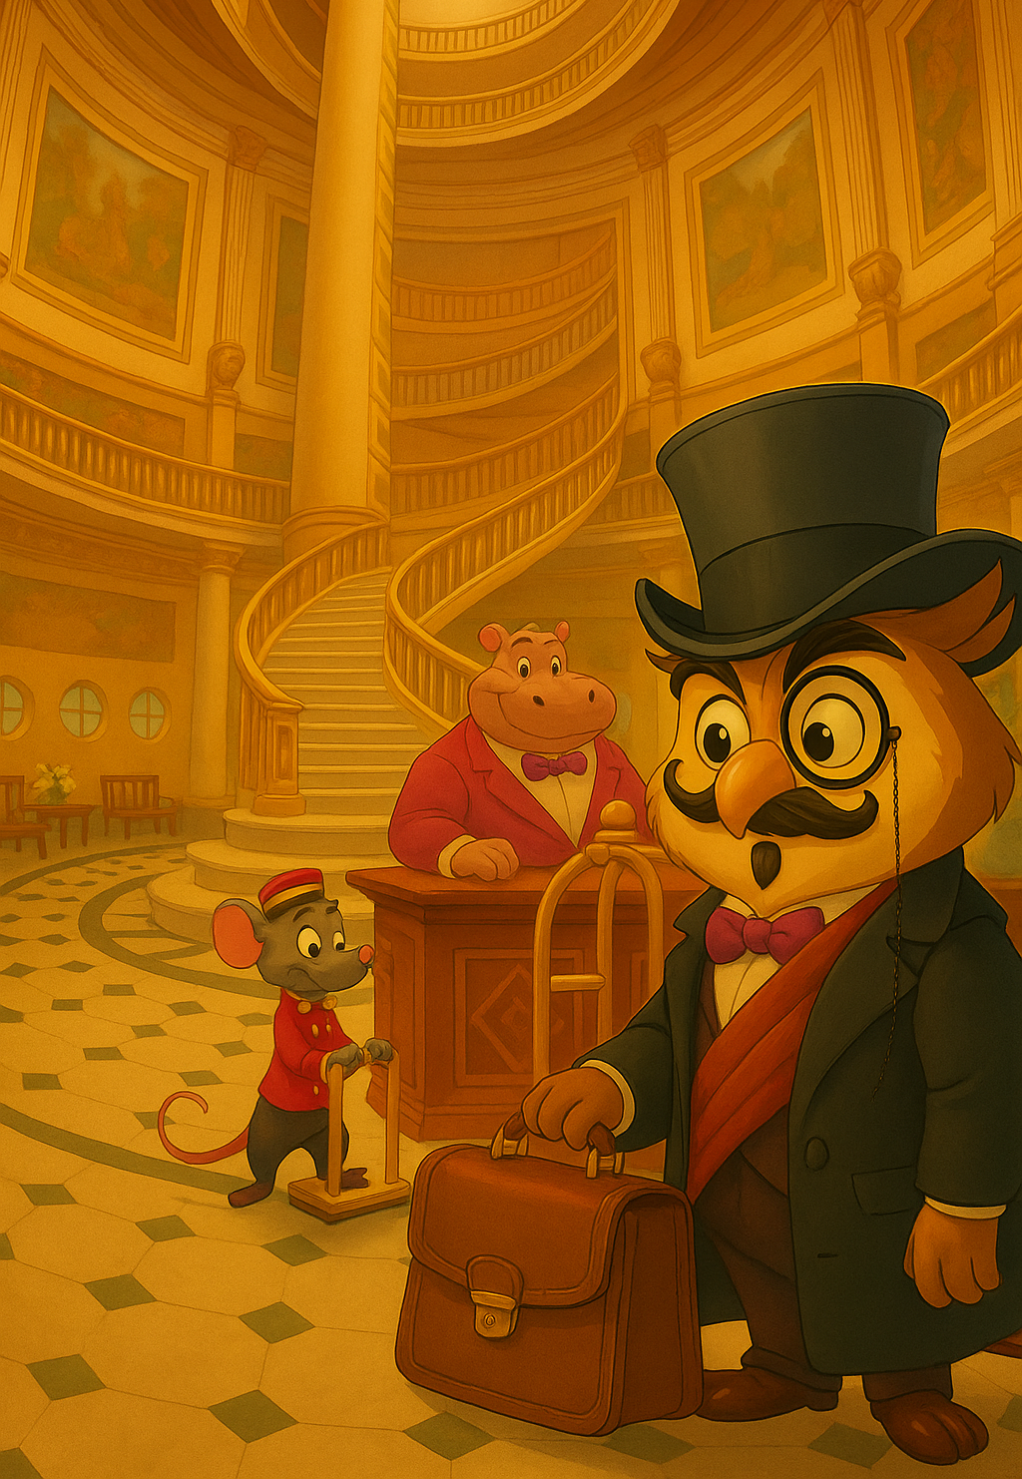
\includepdf[pages={1},
            pagecommand={\thispagestyle{fancy}}, % Apply your custom 'fancy' style
            fitpaper=true,
            noautoscale
           ]{owl.pdf}
\clearpage
\chapter{O Mistério}
Tudo começou quando uma renomada coruja usando chapéu e monóculo chegou.

``É um prazer recebê-lo no Grande Hotel Infinita'', disse Henrietta. ``Um lugar onde a busca incessante se desfaz, para que você descanse e encontre paz.''
%``Um lugar onde a busca incessante fica para trás, onde você pode descansar e deixar o redemoinho dos turbulentos sonhos para trás.''

A coruja respondeu com um pedido peculiar: ``Obrigado, minha cara. Eu gostaria de um quarto no primeiro andar, pois tenho um medo terrível de altura.''

``Os quartos do primeiro andar estão completamente cheios'', suspirou Henrietta. Era um problema comum, já que os hóspedes geralmente não gostavam de ter que usar as escadas. Mas, tentando ser o mais amigável e cuidadosa possível, ela acrescentou, ``Mas não se preocupe!''

Para acomodar este hóspede eminente, ela ligou para o distinto leão-marinho e, da maneira mais delicada, pediu-lhe que se mudasse do Quarto 1 no primeiro andar para o Quarto 1 no segundo andar. O leão-marinho prontamente concordou.

\vfill
\begin{center}
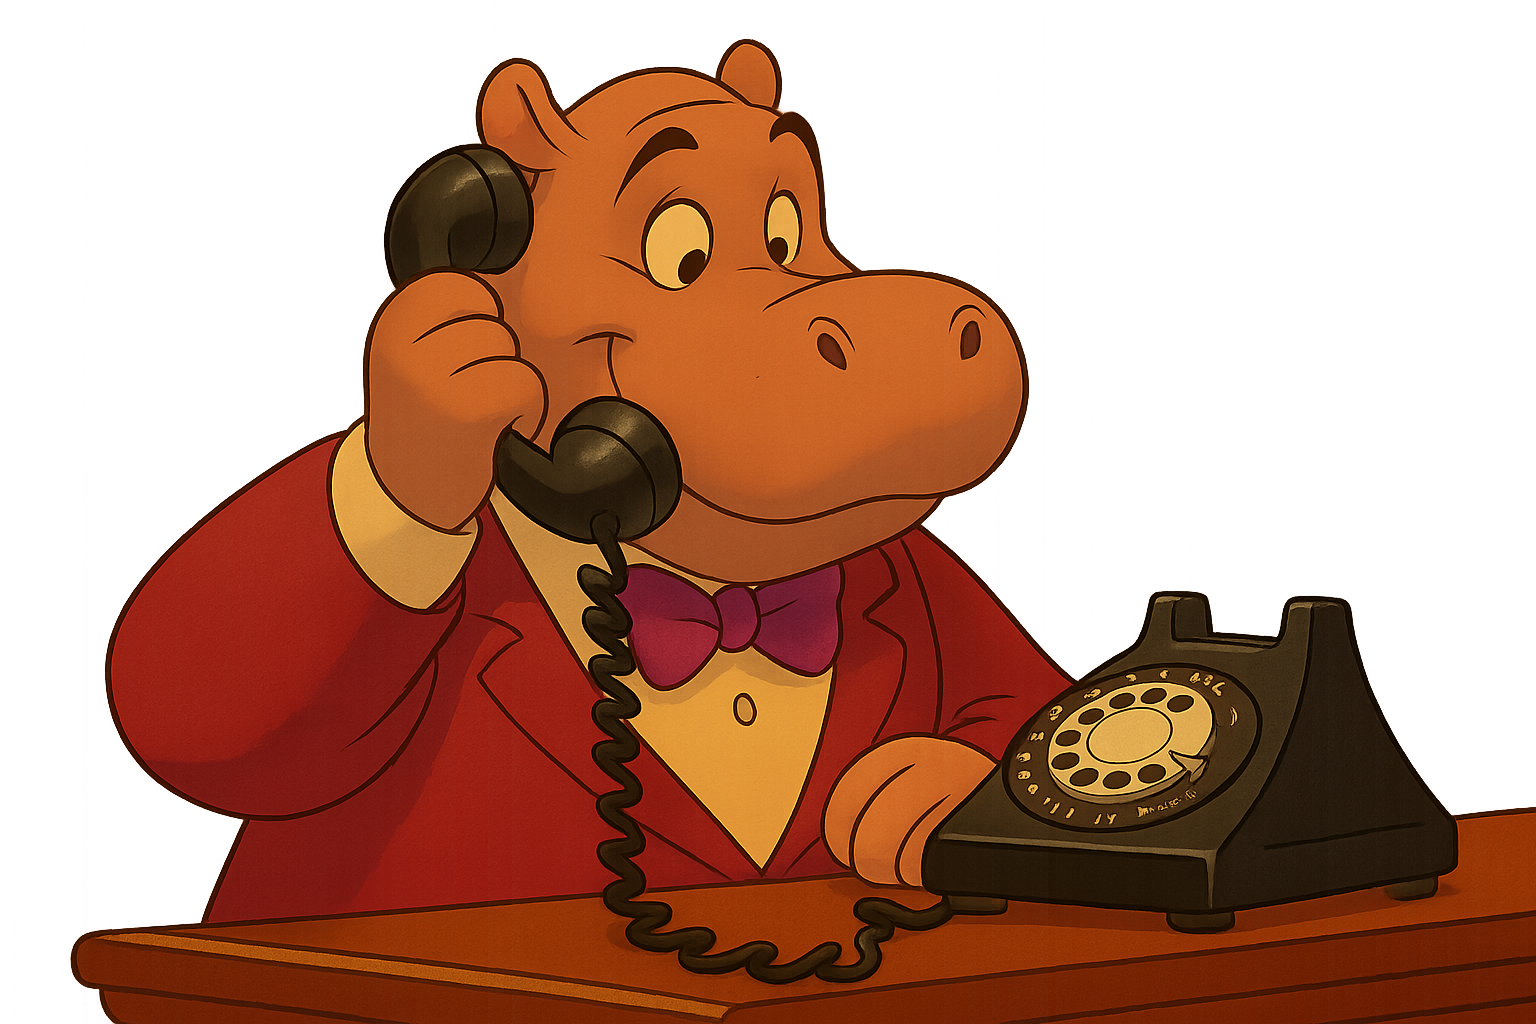
\includegraphics[width=0.5\textwidth]{images/telephone.png}
\end{center}

\clearpage
\includepdf[pages={1},
            pagecommand={\thispagestyle{fancy}}, % Apply your custom 'fancy' style
            fitpaper=true,
            noautoscale
           ]{elevator.pdf}

%Para acomodar este hóspede eminente, ela chamou o distinto leão-marinho e, da maneira mais delicada, pediu-lhe que se mudasse do Quarto 1 no primeiro andar para o Quarto 1 no segundo andar. O leão-marinho prontamente concordou. 
Bernard rapidamente pegou os pertences do leão-marinho e os moveu para o andar de cima usando o pequeno elevador de carga.

``Bernard irá ajudá-lo a chegar ao seu novo quarto imediatamente!'' acrescentou Henrietta.

A coruja ficou encantada em pegar o quarto recém-vago no primeiro andar, e Bernard rapidamente trouxe sua bagagem.

Poucos minutos depois, uma graciosa girafa de cachecol e meias compridas apareceu. Com um olhar deslumbrante, ela entrou, observando cada detalhe do grande hotel, e com a cabeça erguida, quase a bateu no lustre central. Bernard, vendo Henrietta se preparando para mover a coruja, sugeriu: ``Vamos mover o hóspede do Quarto 2! A coruja acabou de se acomodar e tem medo de altura.'' Henrietta concordou. A girafa, mostrando-se agradecida, disse: ``Que gentileza a sua! Assim não precisarei me esforçar subindo e descendo as escadas infinitas!'' Bernard rapidamente pegou os pertences dela, e ela se acomodou feliz em seu novo quarto.

\vfill
\begin{center}
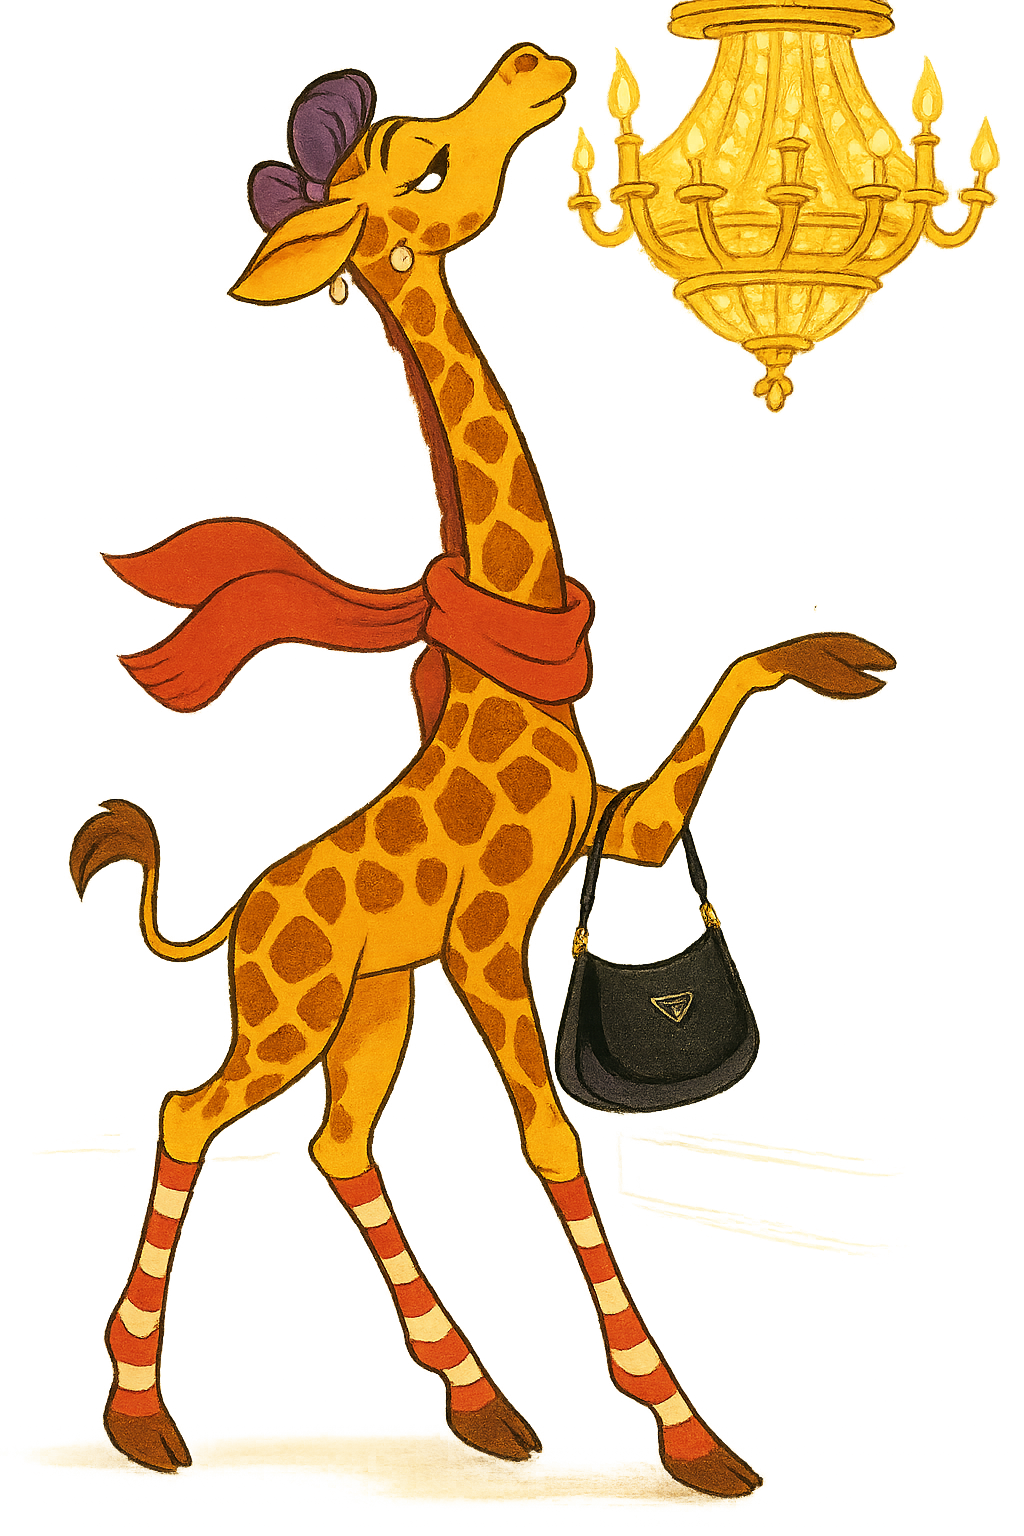
\includegraphics[width=0.45\textwidth]{images/giraffe.png}
\end{center}

\clearpage
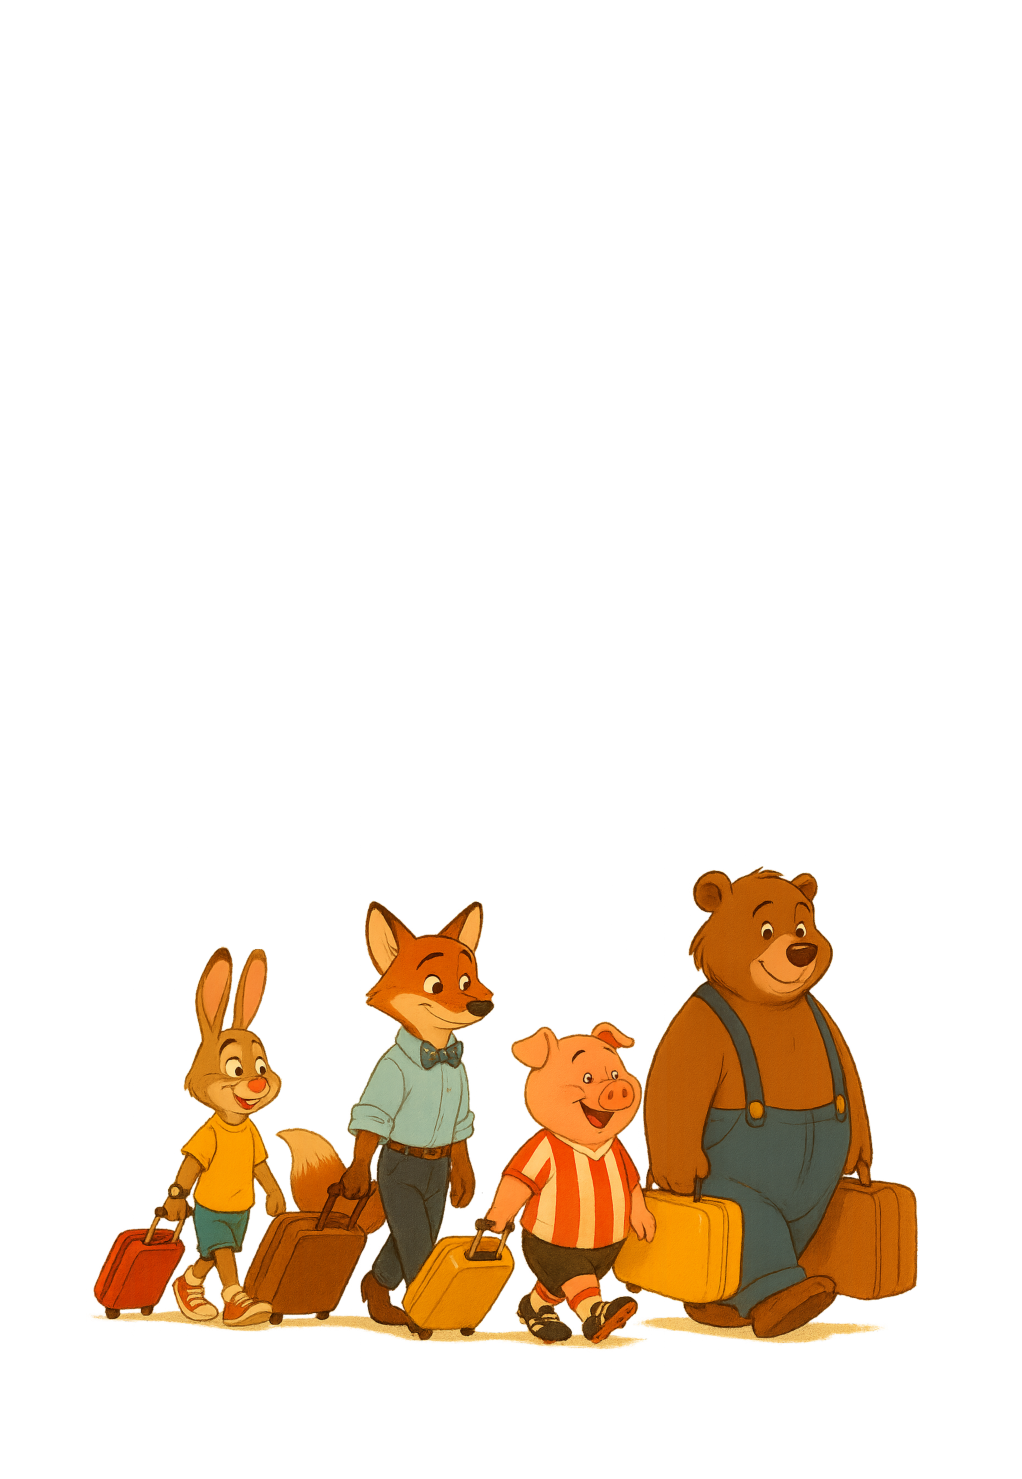
\includepdf[pages={1},
            pagecommand={\thispagestyle{fancy}}, % Apply your custom 'fancy' style
            fitpaper=true,
            noautoscale
           ]{checkinanimals.pdf}

Ao longo do dia, mais e mais hóspedes animais chegaram: um coelho com um relógio de pulso, uma raposa com uma gravata-borboleta, um porco com chuteiras de futebol e um urso com suspensórios. Cada vez, Bernard e Henrietta repetiam seu sistema inteligente, movendo o próximo hóspede do primeiro andar para o segundo, sempre para o mesmo número de quarto. Era uma solução engenhosa para um problema peculiar. No final do dia, eles haviam recebido um total de 54.907 novos hóspedes, e parecia que todos estavam bem acomodados... mas era apenas o início de uma noite caótica.



\clearpage
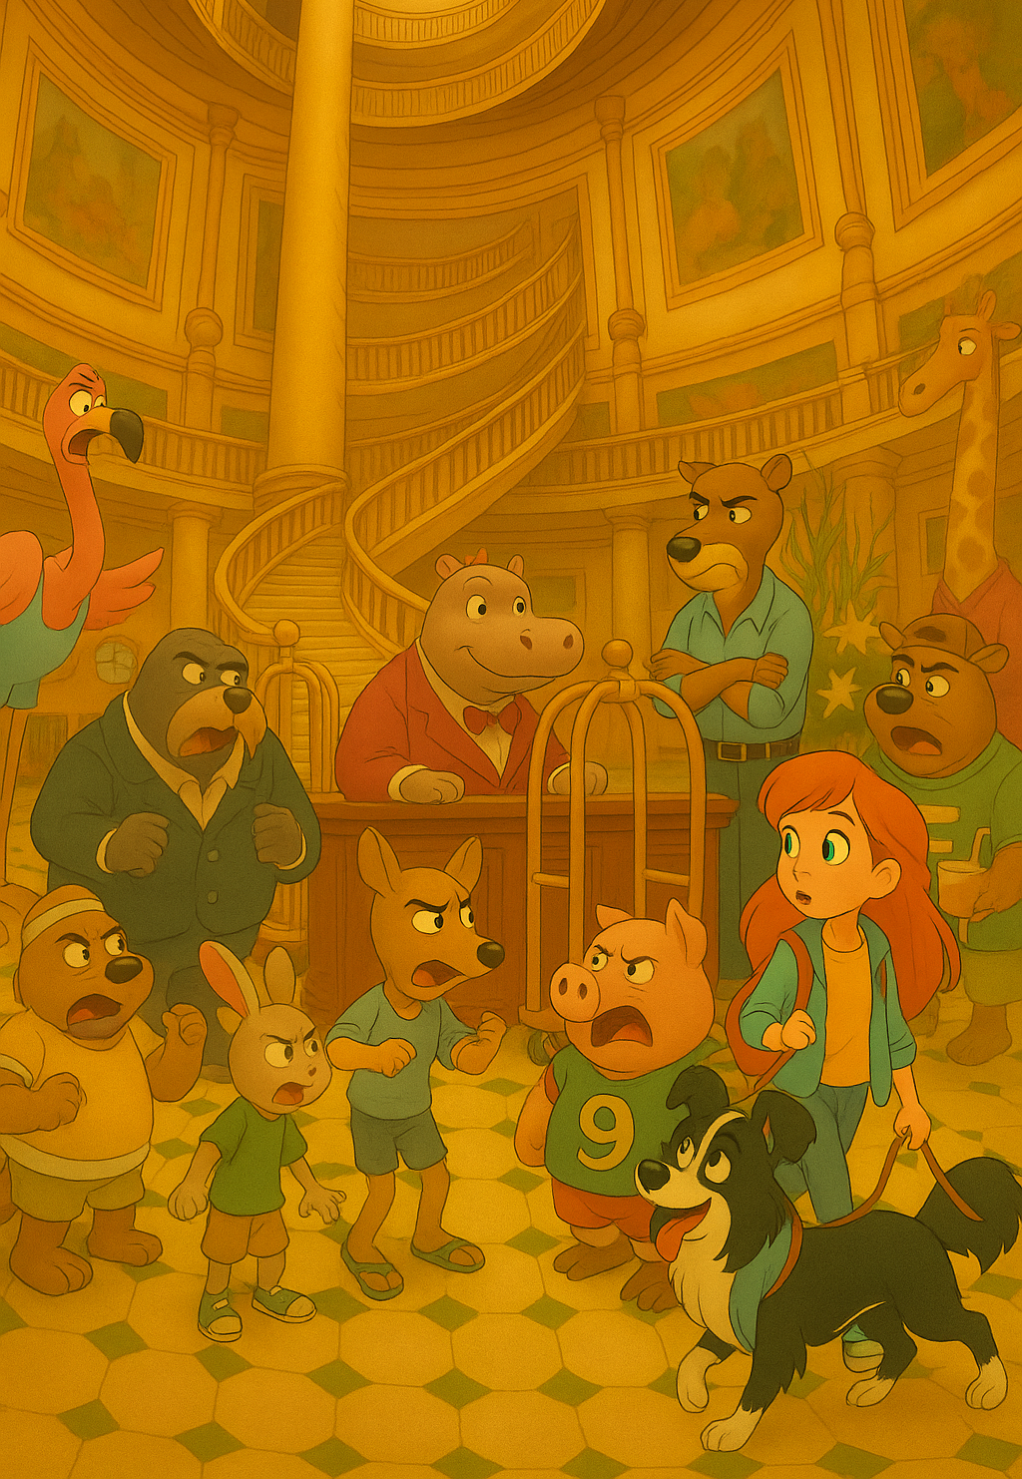
\includepdf[pages={1},
            pagecommand={\thispagestyle{fancy}}, % Apply your custom 'fancy' style
            fitpaper=true,
            noautoscale
           ]{fuss.pdf}
\clearpage
\chapter{As Pistas}
Quando o sol se pôs, os hóspedes que estavam passeando pela cidade começaram a voltar para o hotel. O leão-marinho estava na recepção, seus longos bigodes caídos. ``Meu cachimbo sumiu!'', ele berrou. ``Foi um presente que ganhei quando me tornei membro honorário do Clube de Bocha do Ártico.'' A coruja grasnou em desespero, segurando uma foto de seu avô. ``Meu monóculo sumiu! É a única coisa que me resta dele!'' A girafa chorou que seu cachecol vermelho havia desaparecido. ``É a única lembrança da minha primeira vez esquiando no Himalaia!'' O coelho pulava para cima e para baixo, procurando seu relógio de pulso. ``Eu preciso desesperadamente do meu relógio! Como vou saber agora quando é a hora do meu remédio?!'' O porco suava de ansiedade. ``Meu jogo de futebol está prestes a começar!'' E bem atrás dele estava um urso, que segurava as calças com as patas. ``Meus suspensórios sumiram!'', ele rosnou. ``Como minhas calças vão ficar no lugar sem eles?''

A girafa, visivelmente aborrecida, acrescentou: ``Precisamos encontrar o ladrão! Eles não podem roubar nossos objetos de valor e sair impunes!'' Sua frustração foi ecoada pelos outros, todos ansiosos para resolver o crime.

O coelho, aproveitando a determinação de todos, apontou: ``Quando desci para a farmácia, vi o lobo perambulando pelas escadas e corredores.'' Foi então que o lobo apareceu e, com uma tosse engasgada, disse em voz alta: ``Cof! Ei! Eu também sou uma vítima aqui! Estava perambulando por aí procurando meu vale-spa, que ganhei na recepção!''

Henrietta interveio rapidamente, pedindo a todos que se acalmassem. ``O Sr. Lobo foi de fato premiado com um vale-spa na sua chegada.''

Então, a avestruz apareceu, segurando um bilhete em seu bico. ``Acho que encontrei seu vale, Sr. Lobo.''

\begin{center}
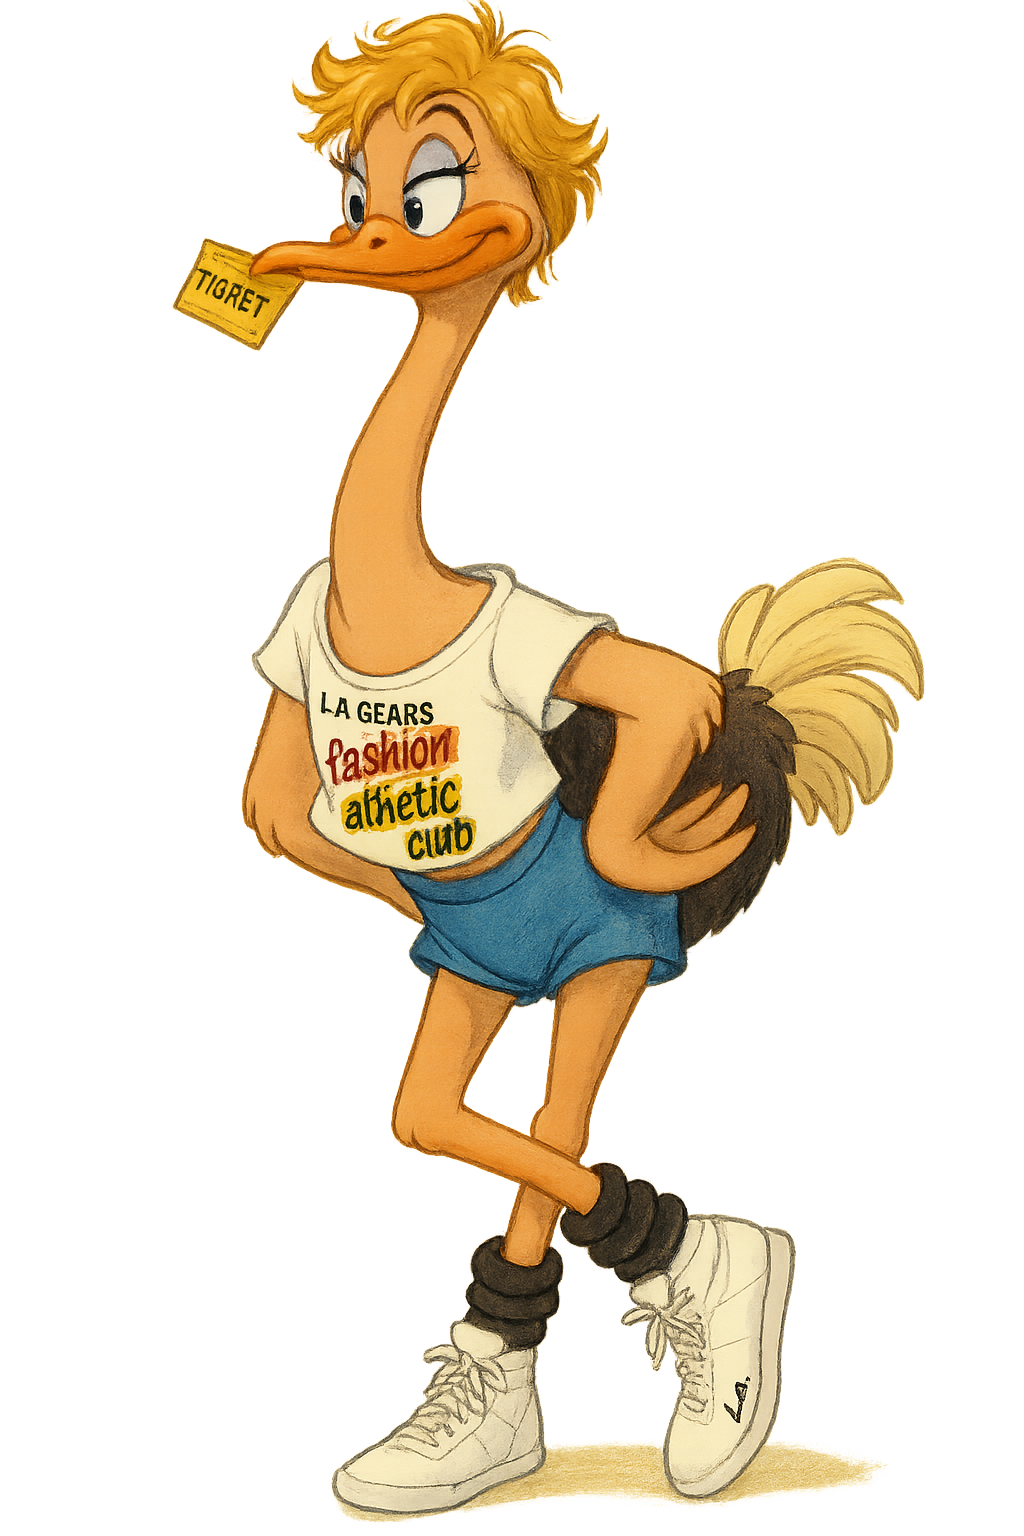
\includegraphics[width=0.2\textwidth]{images/ostrich.png}
\end{center}

O coelho, com um olhar astuto, apontou: ``Podemos então concluir que o lobo não foi uma vítima dos desaparecimentos...''

Os animais começaram a se voltar uns contra os outros. A coruja acusou o coelho de ser muito esperto e inquieto. Além disso, ela acrescentou, ``Ele está apontando o dedo para o lobo para tirar o foco de si mesmo.'' O coelho retrucou, ``Isso é uma acusação leviana!'' Nesse momento, um galo de crista vermelha, aproveitou a confusão e cantou em voz alta: ``Não confiem nela!'' Ele apontou a asa para a raposa, acusando-a de ser muito astuta e sorrateira. A raposa, por sua vez, apontou a pata para o porco, alegando que ele era desajeitado e bagunceiro. O porco, frustrado, apenas bufou em descrença.

Quando a confusão atingiu seu auge, uma garota chamada Anne chegou com seu Border collie peludo, Scotch. Ela ouviu atentamente as histórias dos animais, enquanto Scotch, por outro lado, estava cheirando tudo.

``Podemos ajudar'', disse Anne com confiança. ``Scotch pode seguir o rastro dos seus objetos perdidos.''

A raposa e o lobo trocaram um olhar astuto. ``Por que vocês não começam pelo quarto do coelho?'', sugeriu a raposa. ``Ele parece terrivelmente nervoso.''

``Podem ir!'' o coelho exclamou, estufando o peito. ``Podem ver meu quarto. Eu não tenho nada a temer, e vocês vão se decepcionar!''

Todos foram para o quarto do coelho. Scotch começou a cheirar tudo: a porta, o chão, o guarda-roupa... e de repente, eles viram um monóculo brilhante caído no chão, ao lado do elevador de carga. O lobo soltou um bufo satisfeito. ``Bem, parece que encontramos o que estávamos procurando.''

\clearpage
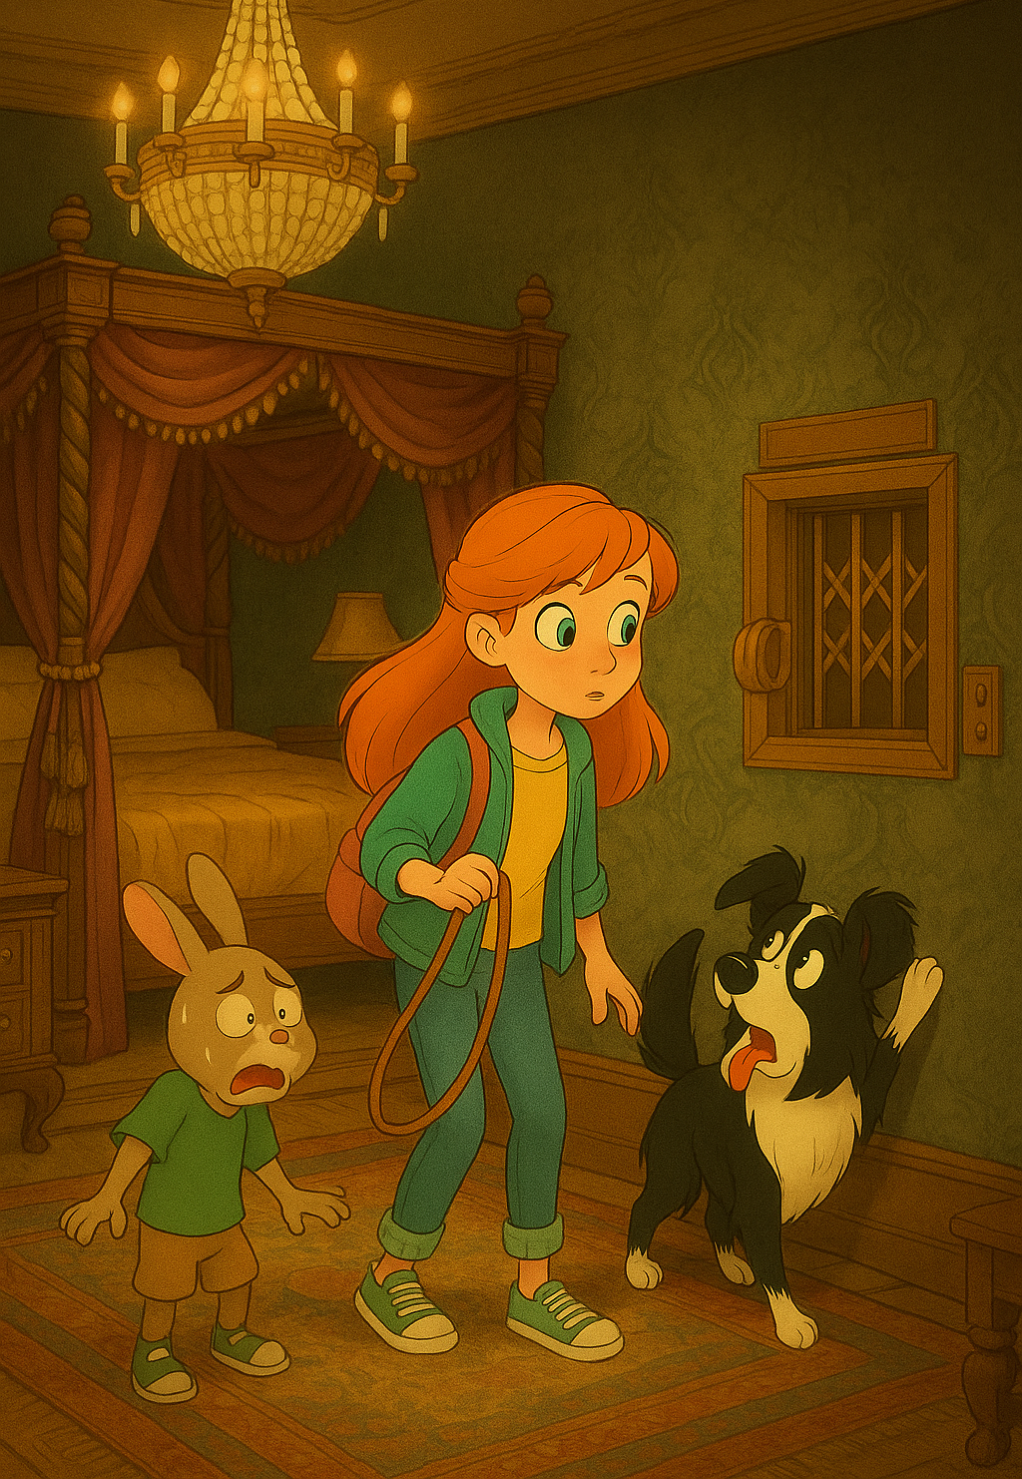
\includepdf[pages={1},
            pagecommand={\thispagestyle{fancy}}, % Apply your custom 'fancy' style
            fitpaper=true,
            noautoscale
           ]{rabbitpanic.pdf}


O coelho gaguejou, ``Eu não sei como isso veio parar aqui!'' Ele suou frio, ficou pálido, e parecia que ia desmaiar.

Mas Scotch latiu mais uma vez. Ele se ergueu sobre as patas traseiras, com as patas dianteiras apoiadas na parede para se equilibrar. Com o nariz levantado, ele cheirou o elevador avidamente, seu corpo tenso de curiosidade e excitação.

``Parece que o rastro leva a este pequeno elevador'', Anne acrescentou. ``Para onde ele vai?''

Bernard respondeu prontamente: ``Ele vai para todos os quartos do hotel.''

Henrietta acrescentou: ``Mas há um número infinito de quartos... levará uma eternidade para encontrar os itens perdidos!''

Scotch latiu novamente e começou a puxar Anne para fora do quarto. Ele a conduziu pelo corredor até um carrinho de serviço de quarto que estava parado no meio. Um pano branco cobria os itens na prateleira inferior, mas o nariz de Scotch estava trabalhando a todo vapor. Com o cão curioso cheirando com afinco, Anne levantou o pano com cuidado para ver o que havia por baixo.

Ela ficou surpresa ao encontrar um pote cheio de biscoitos de cachorro. Ela riu, ``Haha! Scotch, seu guloso!''

Nesse momento, Bernard se aproximou, abriu o pote e lhe deu três biscoitos. Scotch latiu, como se estivesse agradecendo pelo agrado.

%\begin{center}
%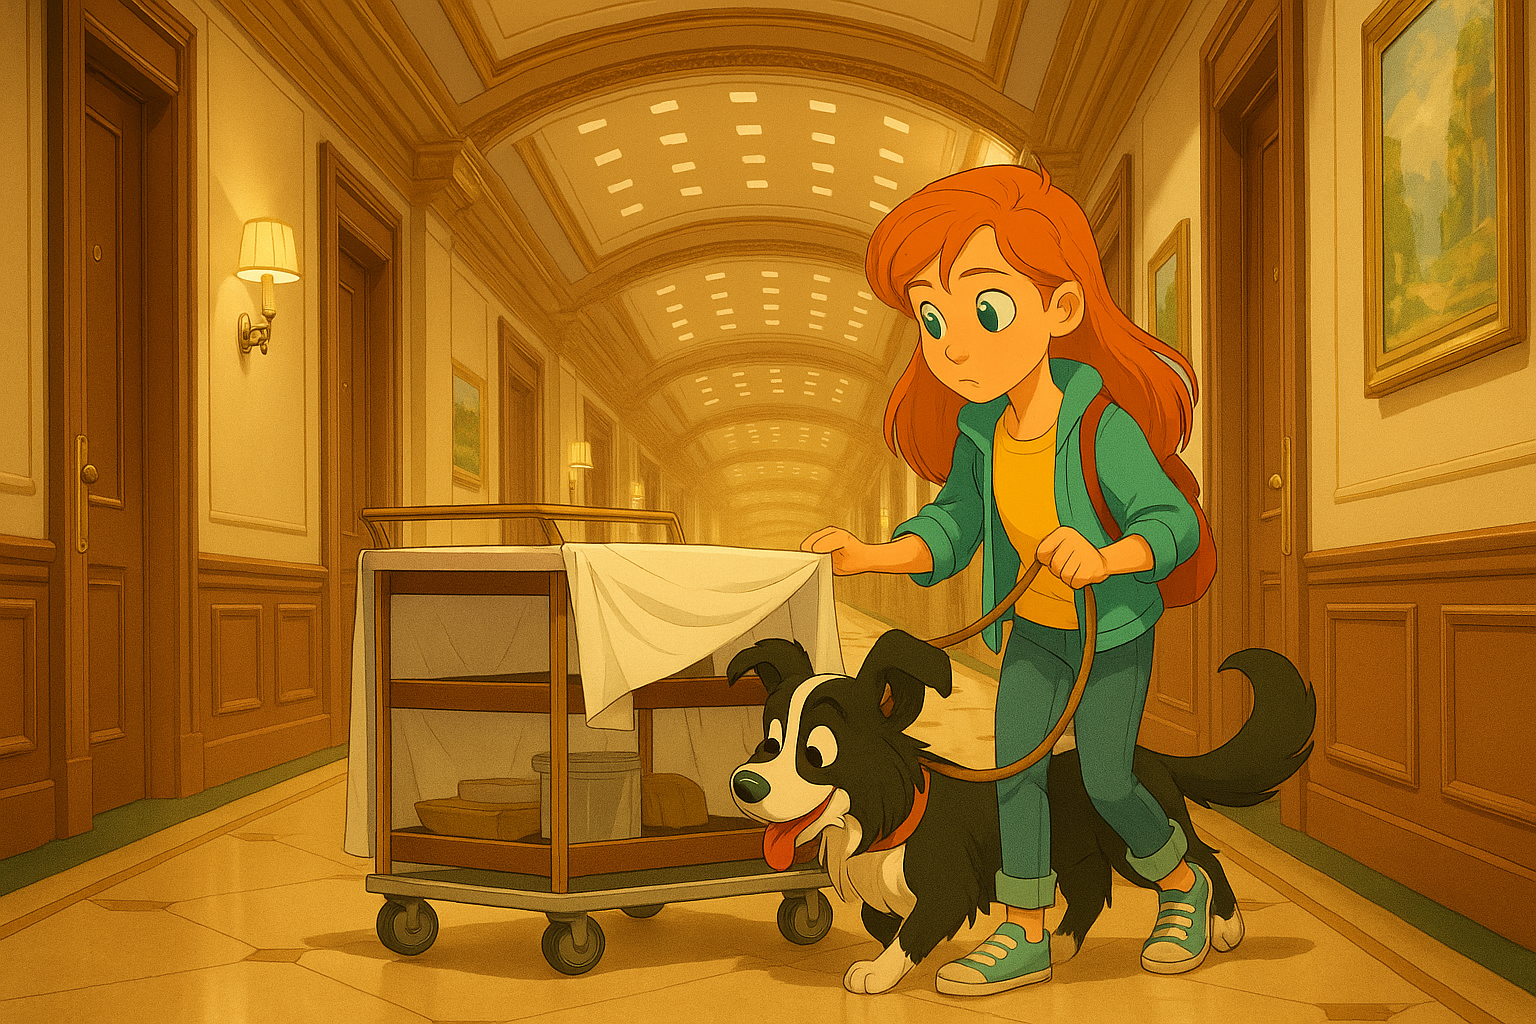
\includegraphics[width=0.55\textwidth]{images/biscuits.png}
%\end{center}

%Após seu merecido lanche, Scotch então disparou de volta para o saguão, com todo o grupo seguindo logo atrás dele. Ele encontrou outra porta para o elevador de carga, sentou e latiu. 
Após seu merecido lanche, Scotch conduziu o grupo. Procuraram quarto após quarto, mas eles não conseguiram encontrar uma única pista. À medida que a esperança dos animais começava a se esvair, a pura impossibilidade da tarefa -- encontrar os itens perdidos nessa infinidade de quartos -- se tornava evidente. Quando eles estavam prestes a voltar para o saguão, Scotch encontrou outra porta para o elevador de carga, sentou e latiu.
Anne olhou da porta para o grupo de animais, com um olhar de quem descobriu a resposta. ``Acho que entendi agora'', ela disse. ``Esta porta leva ao mesmo elevador, não é?''

Bernard imediatamente acrescentou: ``Exato! Para mover os pertences dos hóspedes, precisávamos usar esta entrada para o elevador para que pudéssemos escolher para qual quarto enviá-los.''

\clearpage
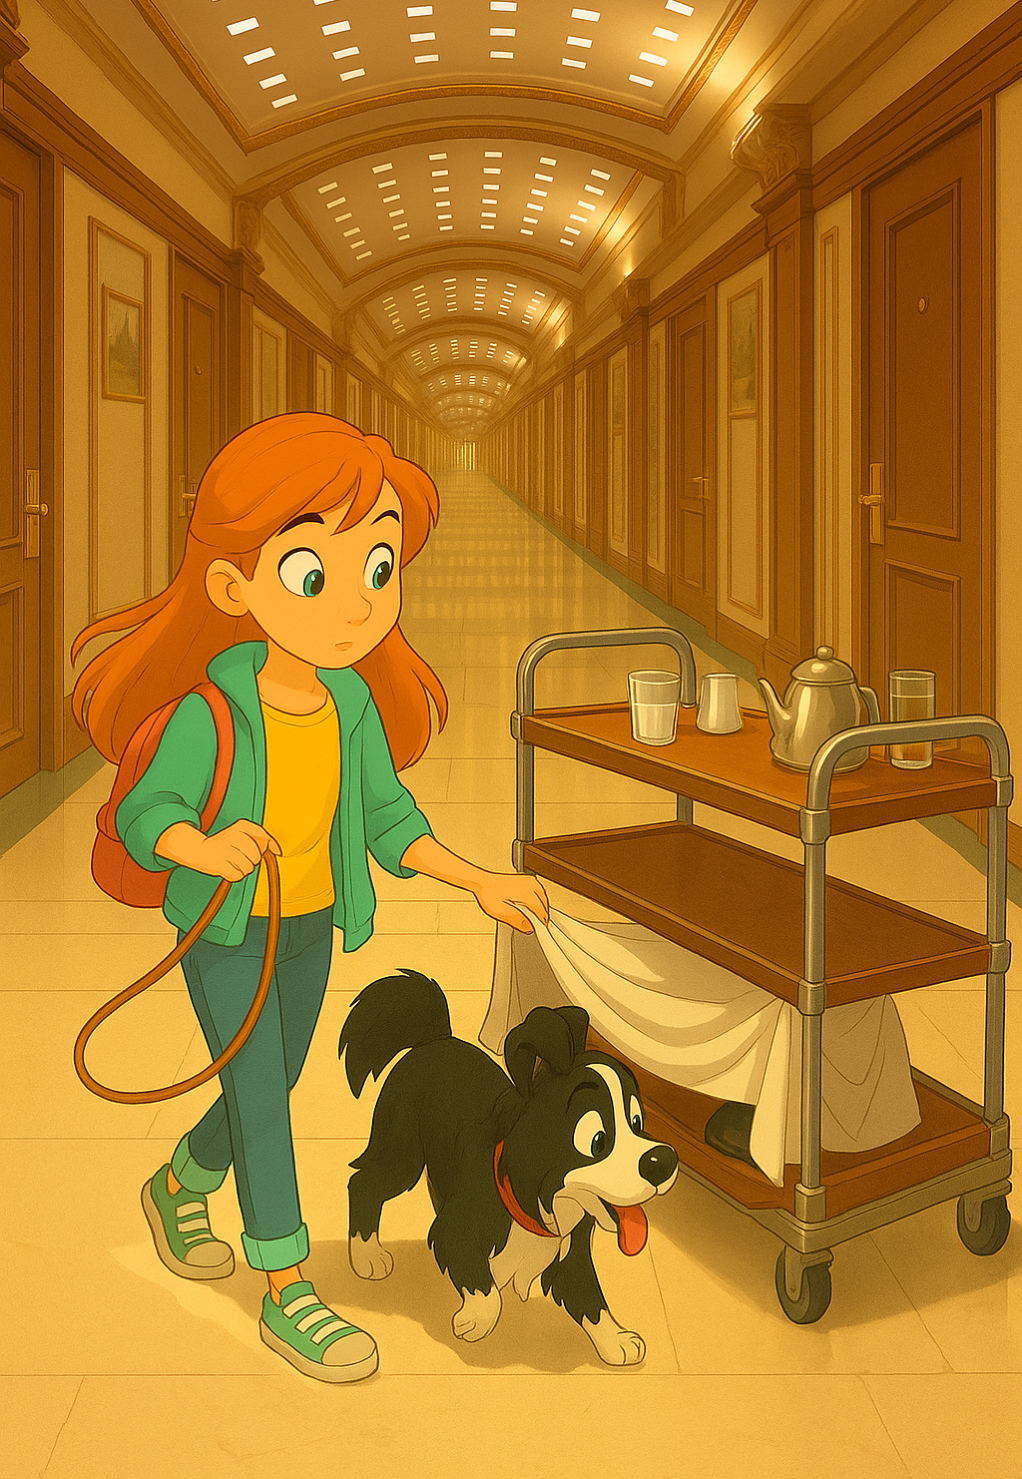
\includepdf[pages={1},
            pagecommand={\thispagestyle{fancy}}, % Apply your custom 'fancy' style
            fitpaper=true,
            noautoscale
           ]{biscuit.pdf}

\clearpage
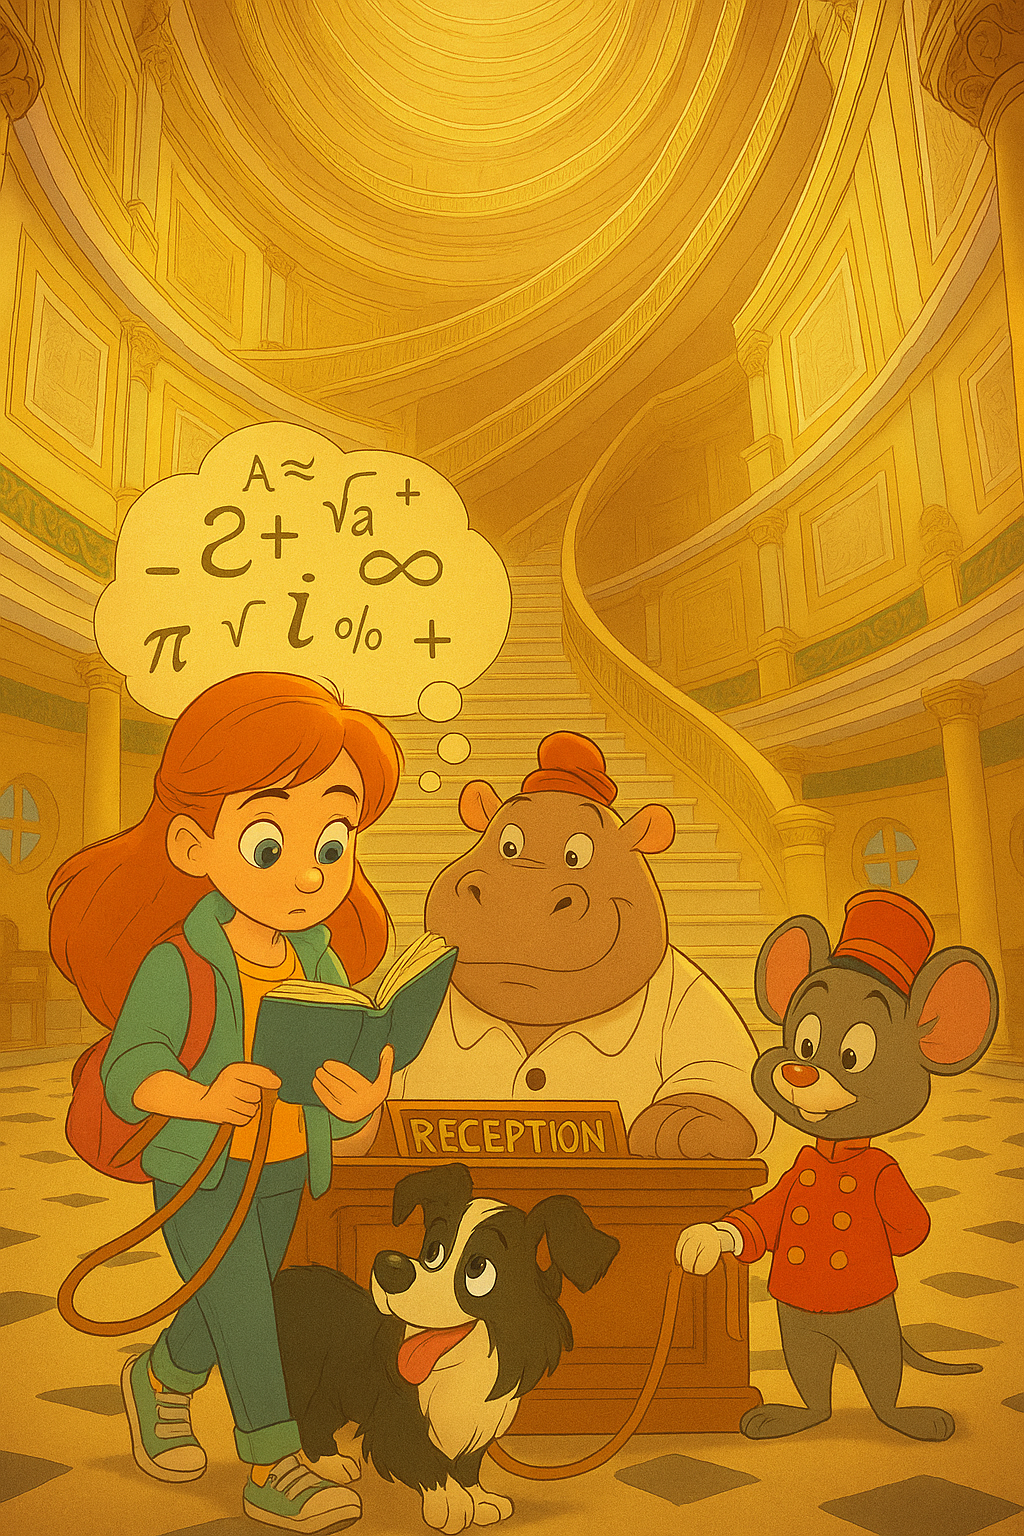
\includepdf[pages={1},
            pagecommand={\thispagestyle{fancy}}, % Apply your custom 'fancy' style
            fitpaper=true,
            noautoscale
           ]{manual.pdf}

Anne apontou, pensativa: ``Está começando a ficar claro. Só precisamos descobrir o funcionamento intrincado do sistema do elevador.''

Bernard perguntou: ``Temos um mapa do sistema do elevador?''

Henrietta explicou que eles só tinham um manual, e Anne comentou: ``Não poderia existir um mapa assim, ou ele seria infinitamente grande!'' Bernard quase riu e disse: ``Vou procurar o manual. Já volto!''

Bernard rapidamente voltou com o manual nas mãos. Ele o entregou a Anne, que imediatamente começou a folhear suas páginas. ``Ah! Achei!'' ela exclamou com entusiasmo. ``Os engenheiros usaram a Função de Emparelhamento de Cantor para mapear o número do quarto e o andar com a posição do elevador em sua trilha infinita.'' 
Ela mostrou a Henrietta uma fórmula no livro, explicando como ela realizava o mapeamento. %mapeava o número do quarto e o andar para um único número que dizia ao elevador para onde ir. 
Ela também alertou: ``Temos que lembrar que o índice aqui começa com zero!''
%Ela mostrou a Henrietta uma fórmula no livro: $n=(i+j)(i+j+1)/2+j$. Anne explicou: ``$n$ é a posição do elevador, $i$ é o número do quarto e $j$ é o andar.'' Ela também alertou: ``Temos que lembrar que o índice aqui começa com zero!''

Todos olharam para Anne com alívio, apesar de não conseguirem entender a matemática que ela usou. Ela abriu a bolsa e pegou uma calculadora científica. Depois de algumas teclas, exclamou: ``Entendi! Vamos, Scotch! Vamos encontrar os tesouros desaparecidos!''


\clearpage
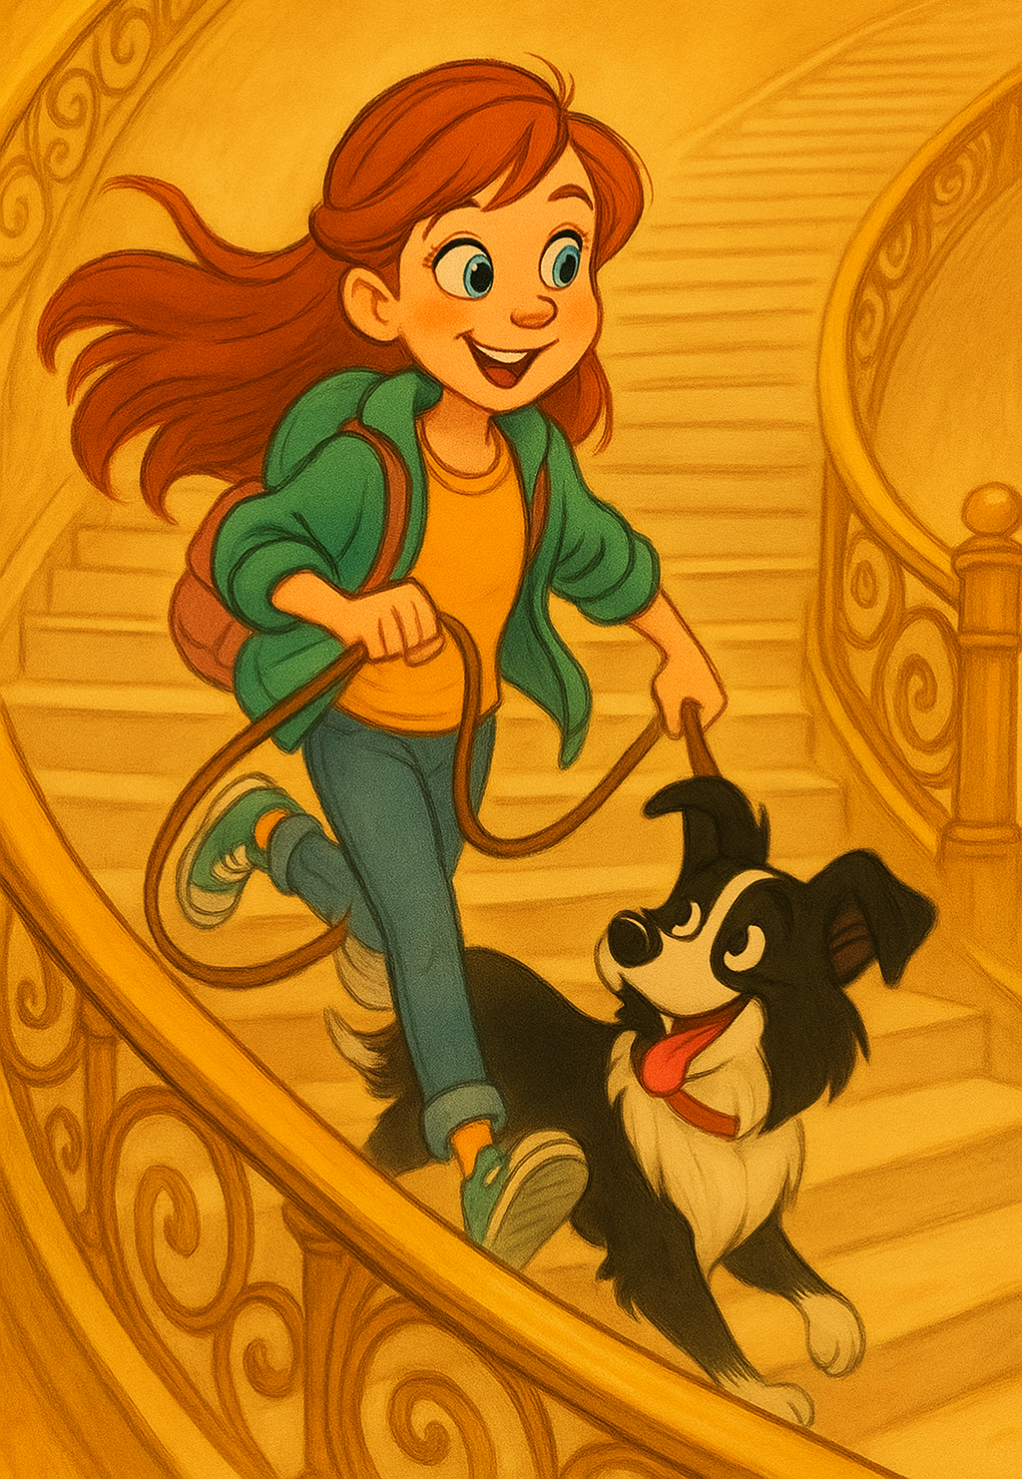
\includepdf[pages={1},
            pagecommand={\thispagestyle{fancy}}, % Apply your custom 'fancy' style
            fitpaper=true,
            noautoscale
           ]{running.pdf}
\clearpage
\chapter{O Encontro}
Scotch latiu e começou a correr, puxando Anne. Ele estava claramente animado! Eles subiram as escadas e, subindo, subindo, subindo, passaram por inúmeros quartos e correram de um andar para outro. Eles visitaram um quarto específico e encontraram o cachimbo perdido do leão-marinho. Subindo as escadas novamente, eles encontraram o cachecol, depois o relógio, as chuteiras de futebol, e os suspensórios do urso. Após um tempo finito, visitando um número contável de quartos em muitos andares diferentes, todos os itens preciosos foram finalmente recuperados. 

\clearpage
\includepdf[pages={1},
            pagecommand={\thispagestyle{fancy}}, % Apply your custom 'fancy' style
            fitpaper=true,
            noautoscale
           ]{findingitens.pdf}

O mistério dos tesouros perdidos foi resolvido! O leão-marinho, com um sopro em seu cachimbo, declarou que Anne era membro honorária do Clube de Bocha do Ártico por seu raciocínio rápido. A coruja a presenteou com um marcador de livro dourado como sinal de reconhecimento por suas habilidades notáveis. A girafa a convidou para uma temporada de esqui nos Alpes. O coelho tomou seu remédio, pois já estava atrasado, e depois de sentir alívio, deu um abraço caloroso em Anne. O urso, agora feliz usando seus suspensórios, soltou um grito de alegria e deu alguns biscoitos caninos para Scotch, como agradecimento por sua ajuda em resolver o enigma. Henrietta ofereceu a Anne uma noite grátis no hotel. Bernard disse que nunca mais se esqueceria de verificar se o elevador de carga estava completamente vazio antes de enviar os pertences de um novo hóspede. E o porco... bem, ele saiu correndo sem se despedir, porque seu jogo de futebol já havia começado.

\vfill
\begin{center}
\Huge
FIM
\end{center}


\clearpage

\includepdf[pages={1},
            pagecommand={\thispagestyle{fancy}}, % Apply your custom 'fancy' style
            fitpaper=true,
            noautoscale
           ]{spa.pdf}
\clearpage
\chapter*{Posfácio}
O paradoxo que Henrietta e Bernard tentaram resolver é uma ideia do famoso matemático David Hilbert. Ele propôs um experimento mental: como um hotel infinito, com todos os quartos ocupados, pode acomodar um novo hóspede? A solução dele era simples: mude o hóspede do quarto $n$ para o quarto $n+1$, o que libera o quarto 1 para o novo hóspede. Para acomodar um número infinito de novos hóspedes, ele sugeriu mover o hóspede do quarto $n$ para o quarto $2n$, o que libera todos os quartos de número ímpar para os novos hóspedes.

Nossa história estende essa ideia para duas dimensões, criando um hotel com um número infinito de andares e infinitos quartos em cada andar. Isso faz com que o problema pareça ainda mais impossível! Como um único elevador poderia visitar cada quarto, um por um?

A solução de Anne, usando a função de pareamento de Cantor, nos mostra algo incrível sobre o infinito. Intuitivamente, parece que um hotel com um número infinito de andares e um número infinito de quartos por andar ($\mathbb{N}\times\mathbb{N}$) seria muito, muito maior do que uma única lista infinita de números ($\mathbb{N}$) que representa a posição do elevador de carga em seu trilho infinito para visitar os quartos. Mas a função de Cantor mostra uma bijeção -- uma correspondência um-para-um -- entre esses dois conjuntos, provando que eles têm o mesmo tamanho.

O matemático Georg Cantor provou que esses dois infinitos são, na verdade, do mesmo tamanho. Ele chamou essa ``tamanho'' de cardinalidade, e a do infinito contável (como os números naturais) é chamada de Aleph-zero ($\aleph_0$). A função que Anne usou faz a mágica: ela pega um par de números (como o número do quarto e do andar, $(i,j)$) e o transforma em um único número (a posição do elevador, $n$). 
$$n=(i+j)(i+j+1)/2+j$$
O que é ainda mais incrível é que ela pode ser revertida para encontrar o par original. O mapeamento usado por Anne é mostrado na figura abaixo:

\begin{center}
%\documentclass[tikz,border=2mm]{standalone}
%\usepackage{amsmath}
%\usepackage{tikz}
%\usetikzlibrary{arrows.meta, decorations.pathmorphing}
%\begin{document}
\begin{tikzpicture}[
    >=Latex, 
    node style/.style={circle, fill=red, inner sep=2pt, font=\bfseries\sffamily, text=white},
    label style/.style={font=\sffamily},
    grid style/.style={line width=0.5pt, gray!40},
    path style/.style={line width=1.5pt, blue, ->},
    dashed path style/.style={line width=1.5pt, blue, dashed, ->}
]

% Draw the grid
\draw[grid style] (0,0) grid (4,4);

% Draw the axes and labels
\draw[->] (0,0) -- (4.5,0) node[right, label style] {i (número do quarto)};
\draw[->] (0,0) -- (0,4.5) node[above, label style] {j (número do andar)};

% Draw the nodes for the grid points
\foreach \x in {0,1,2,3,4} {
    \foreach \y in {0,1,2,3,4} {
        \node[node style, label={[label style]above right:}] at (\x, \y) {};
    }
}

% Add labels for the axes values
\foreach \i in {0,1,2,3,4} {
    \node[below=15pt, label style] at (\i,0) {\i};
}
\foreach \j in {0,1,2,3,4} {
    \node[left=10pt, label style] at (0,\j) {\j};
}

% Define the path based on the Cantor pairing function
% Path for n=0 to n=10
%\draw[path style] (0,0) -- node[above, pos=0.5, font=\sffamily] {0} (0,0.1);
\draw[path style] (0,0) -- (1,0) node[below, pos=0, font=\sffamily] {0};
\draw[path style] (1,0) -- (0,1) node[below, pos=0, font=\sffamily] {1};
\draw[path style] (0,1) -- (2,0) node[left, pos=0, font=\sffamily] {2};
\draw[path style] (2,0) -- (1,1) node[below, pos=0, font=\sffamily] {3};
\draw[path style] (1,1) -- (0,2) node[left, pos=0, font=\sffamily] {4};
\draw[path style] (0,2) -- (3,0) node[left, pos=0, font=\sffamily] {5};
\draw[path style] (3,0) -- (2,1) node[below, pos=0, font=\sffamily] {6};
\draw[path style] (2,1) -- (1,2) node[right, pos=0.05, font=\sffamily] {7};
\draw[path style] (1,2) -- (0,3) node[left, pos=0, font=\sffamily] {8};
\draw[path style] (0,3) -- (4,0) node[left, pos=0, font=\sffamily] {9};
\draw[path style] (4,0) -- (3,1) node[below, pos=0, font=\sffamily] {10};
\draw[dashed path style] (3,1) -- (2,2) node[right, pos=0.05, font=\sffamily] {11};
\draw[dashed path style] (2,2) -- (1,3);% node[above, pos=0.5, font=\sffamily] {13};
\draw[dashed path style] (1,3) -- (0,4);% node[above, pos=0.5, font=\sffamily] {14};
%\draw[path style] (0,4) -- (4,1) node[above, pos=0.5, font=\sffamily] {15};
%\draw[path style] (4,1) -- (3,2) node[above, pos=0.5, font=\sffamily] {16};
%\draw[path style] (3,2) -- (2,3) node[above, pos=0.5, font=\sffamily] {17};
%\draw[path style] (2,3) -- (1,4) node[above, pos=0.5, font=\sffamily] {18};
%\draw[path style] (1,4) -- (4,2) node[above, pos=0.5, font=\sffamily] {19};
%\draw[path style] (4,2) -- (3,3) node[above, pos=0.5, font=\sffamily] {20};
%\draw[path style] (3,3) -- (2,4) node[above, pos=0.5, font=\sffamily] {21};
%\draw[path style] (2,4) -- (4,3) node[above, pos=0.5, font=\sffamily] {22};
%\draw[path style] (4,3) -- (3,4) node[above, pos=0.5, font=\sffamily] {23};
%\draw[path style] (3,4) -- (4,4) node[above, pos=0.5, font=\sffamily] {24};
\end{tikzpicture}
%\end{document}


\end{center}

%Essa correspondência de um-para-um significa que o conjunto de todos os pares de quartos e andares é, de fato, do mesmo ``tamanho'' que o conjunto de todos os números naturais. É um conceito um pouco difícil de engolir, mas é um dos grandes segredos do infinito!

Essa correspondência um-para-um significa que o conjunto de todos os pares de quartos e andares é, na verdade, do mesmo ``tamanho'' que o conjunto de todos os números naturais. Isso desafia uma de nossas intuições mais básicas. Como o matemático David Hilbert apontou, ao lidar com conjuntos finitos, uma parte é sempre menor do que o todo. Mas, ao lidar com conjuntos infinitos, esse princípio não se aplica mais. Como ele disse: ``Hier gilt nun schon der Satz: ,,Der Teil ist kleiner als das Ganze'' nicht mehr.'' (Hilbert, 1925 em sua palestra ``\"{U}ber das Unendliche''). É um conceito um pouco difícil de assimilar, mas é um dos grandes segredos do infinito!


\clearpage
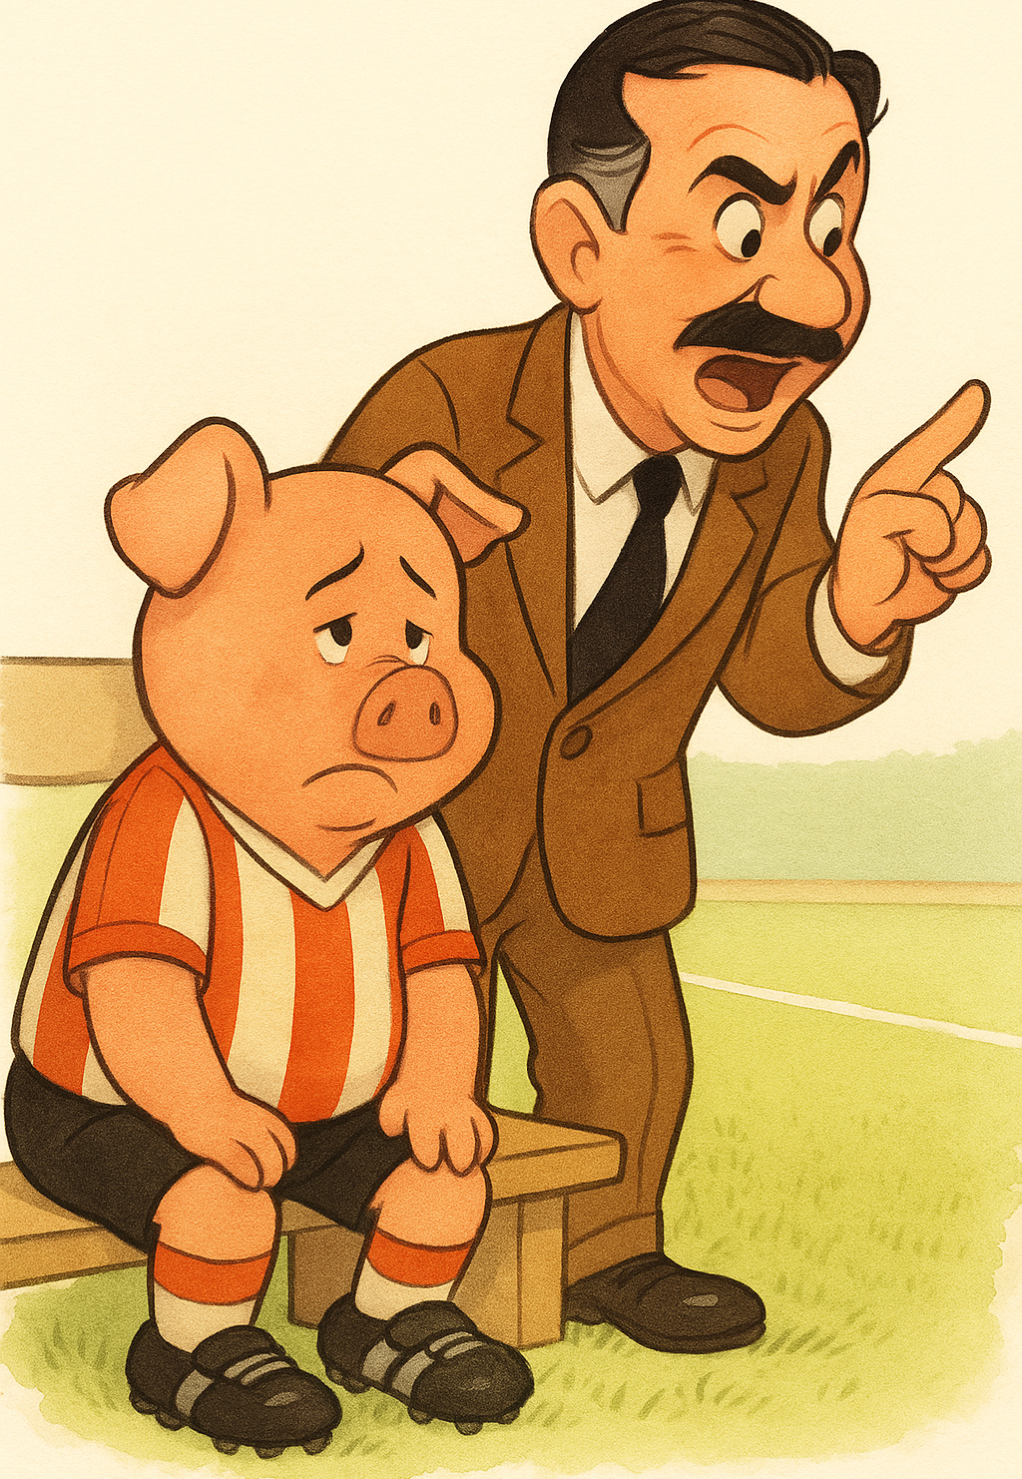
\includepdf[pages={1},
            pagecommand={\thispagestyle{fancy}}, % Apply your custom 'fancy' style
            fitpaper=true,
            noautoscale
           ]{pigfootball.pdf}
\clearpage
\pagenumbering{gobble}
\thispagestyle{empty}
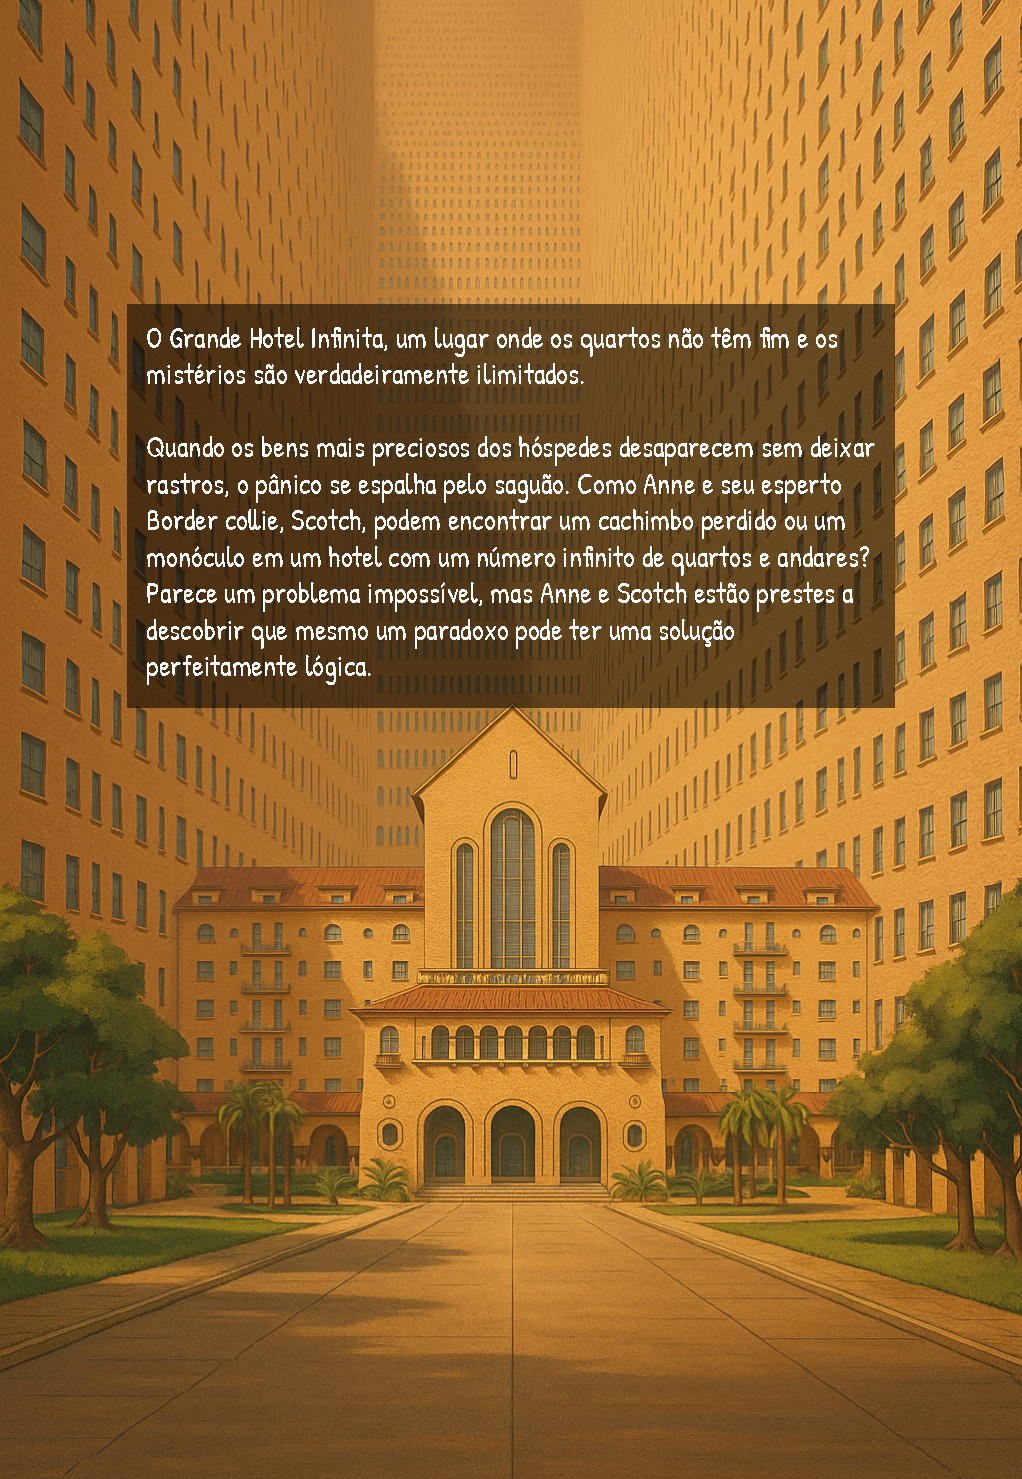
\includepdf[pages=-]{backcover.pt.pdf}

\end{document}
